%        Fil: dokumentation.tex
%     Created: Mon Nov 13 22:45 PM 2011 C
% Last Change: Mon Nov 13 22:45 PM 2011 C
%
\documentclass[11pt,a4paper]{article}

% german dictionary
\usepackage[ngerman]{babel}

% enconding
\usepackage[utf8]{inputenc}

% graphics
\usepackage{graphicx}

% handle positions
\usepackage{float}

% additional math stuff
\usepackage{amsmath,amssymb,environ,esdiff,mathtools}

% set borders
\usepackage{a4wide}

% use URLs
\usepackage{url}

% expand table formatting
\usepackage{array}

% describe algorithms
\usepackage{algorithm}
\usepackage{algorithmic}

% header and footer
\usepackage{fancyhdr}
\pagestyle{fancy}
\fancyhf{}

\fancyhead[L]{Implementation einer Win/Win Strategie für das TSP}
\fancyhead[R]{Semesterarbeit}

\fancyfoot[L]{Andreas Brönnimann}
\fancyfoot[C]{\thepage}
\fancyfoot[R]{\today}
\renewcommand{\footrulewidth}{0.5pt}

% cover
\title {Semesterarbeit\\
Implementation einer Win/Win Strategie für das TSP\\}
\author {Andreas Brönnimann\\
Hochschule für Technik Zürich\\
Dozent: Dr. Hans-Joachim Böckenhauer}
\date {\today}

\begin{document}

% show all references, even the uncited ones
\nocite{*}

% show cover
\maketitle
\setcounter{page}{0}
\thispagestyle{empty}
\newpage

\tableofcontents
\newpage
\section{Einleitung}
\subsection{Ziel und Vorgehensweise}
Ziel dieser Arbeit ist es, die Win/Win Strategie des Papers "`Structural properties of hard metric TSP inputs"'\cite{moemke11} zu Implementieren. Anschliessend wird die Implementation zur Berechnung verschiedener Problemstellungen verwendet. Das Ergebnis wird mit den theoretisch erwarteten Resultaten verglichen und ausgewertet.

Um ein Verständnis für die Implementation zu entwickeln, werden das Traveling Salesman Problem (TSP oder übersetzt: das Problem des Handlungsreisenden), die Grundlagen von Win/Win Strategien und die verwendeten Algorithmen vorgestellt. 

Danach werden die wichtigsten Teile der Implementation erklärt, bevor dann die Ergebnisse ausgewertet werden. 

\subsection{Abgrenzung}
Diese Arbeit beschränkt sich auf die Implementation der Win/Win Strategie und die Auswertung der Ergebnisse. Neue Algorithmen zu finden ist nicht Teil dieser Arbeit.

\subsection{Motivation}
Mich fasziniert, dass die Problembeschreibung sehr einfach ist, die Lösung jedoch äusserst schwierig.
Ausserdem lassen sich viele Überlegungen mit Papier und Stift aufzeichnen, ohne das ein Computer benötigt wird. 
Abbildung \ref{img:simple_tsp} zeigt ein 6 Städte TSP, eine Mögliche Route ist dabei blau markiert. Offensichtlich ist es nicht die optimale Route. Das Bild zeigt jedoch, wie einfach man das Problem für kleine Instanzen analysieren kann, selbst ohne einen Rechner zu benutzen.

\begin{figure}[H]
        \centering
        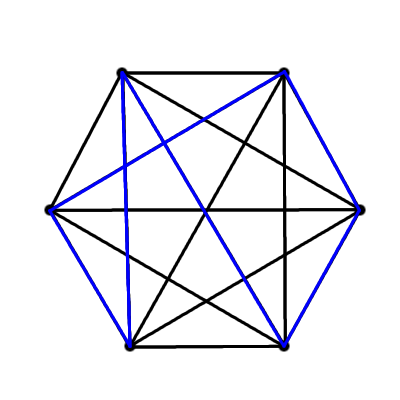
\includegraphics[width=8cm]{gfx/simple_tsp}
        \caption{6 Städte TSP}
        \label{img:simple_tsp}
\end{figure}

\newpage
\section{Traveling Salesman Problem (TSP)}
Dieser Abschnitt gibt einen Überblick zum Traveling Salesman Problem. Als Erstes wird die Problemstellung erklärt und anschliessend der geschichtliche Hintergrund erläutert. Nach einer kurzen Beschreibung zur NP-Vollständigkeit des Problems, wird erklärt, wie das Problem modelliert werden kann. Da es neben dem in dieser Arbeit vorgestellten Algorithmus viele weitere Möglichkeiten gibt, ein TSP zu lösen, werden einige exakte und heuristische Lösungsverfahren kurz beschrieben.

\subsection{Problembeschreibung}
Die Problemstellung ist simple: Es soll eine Rundreise durch eine Anzahl Städte gefunden werden und zwar so, dass der Handlungsreisende wieder an seinen Ausgangspunkt zurückkehrt und die zurückgelegt Strecke möglichst kurz ist.

\subsection{Geschichte}
Der Urheber der Bezeichnung "`Traveling Salesman Problem"' ist nicht genau bekannt. Es ist jedoch klar, dass damit das Auffinden der kürzesten Rundreise eines Handelsreisenden gemeint ist.\footnote{vgl. \cite{applegate06} Seite 1-3} 1983 publizierte Heiner Müller-Merbach in seinem Paper\cite{mueller83} einen Ausschnitt aus dem Buch "`Der Handlungsreisende – wie er sein soll und was er zu thun hat, um Aufträge zu erhalten und eines glücklichen Erfolgs in seinen Geschäften gewiß zu sein – von einem alten Commis-Voyageur"' in dem die Wichtigkeit einer guten Route beschrieben:  
\begin{quotation}
Die Geschäfte führen Handlungsreisende bald hier, bald dort hin, und es lassen sich nicht füglich Reiserouten angeben, die für alle vorkommende Fälle passend sind: aber es kann durch eine zweckmäßige Wahl und Eintheilung der Tour, manchmal so viel Zeit gewonnen werden, dass wir es nicht glauben umgehen zu dürfen, auch hierüber einige Vorschriften zu geben. Ein Jeder möge so viel davon benutzen, als es seinem Zwecke für dienlich hält: so viel glauben wir aber davon versichern zu dürfen, daß es nicht wohl thunlich sein wird, die Touren durch Deutschland in Absicht der Entfernungen und, worauf der Reisende hauptsächlich zu sehen hat, des Hin- und Herreisens, mit mehr Oekonomie einzurichten. Die Hauptsache besteht immer darin: so viele Orte wie möglich mitzunehmen, ohne den nämlichen Ort zweimal berühren zu müssen.
\end{quotation}

Auch wenn das Problem in diesem Buch nicht mathematisch analysiert wird, beschreibt der Text das Traveling Salesman Problem. 

Eine der ersten mathematischen Analysen des Problem stammen aus dem Jahr 1757 vom berühmten Schweizer Mathematiker Leonard Euler. Er veröffentlichte ein Paper, in dem er eine Lösung zur "`Knights Tour"' vorstellte. Bei der "`Knights Tour"' soll auf einem Schachbrett mit dem Springer eine Folge von Sprüngen gefunden werden, so dass jedes Feld genau einmal besucht wird und der Springer am Ende wieder auf seinem Startfeld steht.

Dieses Problem kann als TSP formuliert werden. Die Wegkosten zu den mittels einem Springer erreichbaren Felder sind 0, die Kosten zu den nicht erreichbaren Felder sind 1.\footnote{vgl. \cite{applegate06} Seite 8-10}

\medskip

Einer der bedeutensten frühen Forscher auf dem Gebiet, Merril Flood, sagte in einem Interview, dass der Begriff "`Traveling Salesman Problem"' in den 1930er Jahren als Synonym für das "`48 States Problem"' von Hassler Whitney an der Princeton Universität verwendet wurde. Wer genau die Bezeichnung eingeführt habe, wisse er jedoch nicht.\cite{interview_merrill_flood84}

Abschliessend ist somit nicht auszumachen, wann genau die Forschung auf dem Gebiet des Traveling Salesman Problems begonnen hat.

\medskip

Ein erster Meilenstein im Bezug auf die Lösung des Traveling Salesman Problems gelang George Dantzig, Ray Fulkerson und Selmer Johnson 1954, als sie ein 49 Städte TSP lösen konnten. Die gelöste Instanz beinhaltet Städte aus allen damaligen Bundesstaaten der USA, plus Washington D.C. Das Problem konnte gelöst werden, in dem die Städte Baltimore, Wilmington, Philadelphia, Newark, New York, Hartford und Providence entfernt wurden. Da die Route des neuen TSP durch die entfernten Städte führte, war die optimale Lösung gefunden.

In den 1960er und 1970er beschäftigten sich immer mehr Wissenschaftler mit dem Problem. Richard M. Karp konnte 1972 die NP-Vollständigkeit des Hamiltonkreisproblems beweisen, was die NP-Vollständigkeit des Traveling Salesman Problems impliziert.
%TODO: Quelle

1977 wurde ein 120 Städte TSP von Martin Grötschel gelöst. Die Route beinhaltete Städte im damaligen Westdeutschland.

Im Jahre 1987 wurden gleich drei bedeutende Instanzen gelöst: Ein 532 Städte TSP von Padberg und Rinaldi, ein 666 Städte TSP von Grötschel und Holland und das 2392 Städte TSP, wiederum von Padberg and Rinaldi.\footnote{vgl. \cite{applegate06} S. 50-51}

Anfang der 1990er Jahre begannen David Applegate, Robert E. Bixby, Vašek Chvátal und William J. Cook mit der Entwicklung von Concorde. Seit 1992 wurden immer grössere Instanzen mit Hilfe von Concorde gelöst. Die grössten Erfolg von 1992-2006 sind in Tabelle \ref{tab:concorde_history} ersichtlich.\footnote{\cite{applegate06} Seite 53}

        \begin{table}[H]
                \centering
                \begin{tabular}{| l | r | l |}
                    \hline
                        Jahr    & Anzahl Städte & Bemerkung                 \\ \hline
                        1992    & 3'038         &                           \\ \hline
                        1993    & 4'461         &                           \\ \hline
                        1994    & 7'397         &                           \\ \hline
                        1998    & 13'509        &                           \\ \hline
                        2001    & 15'112        &                           \\ \hline
                        2004    & 24'978        &                           \\ \hline
                        2004    & 33'810        & Concorde mit Domino Party \\ \hline
                        2006    & 85'900        & Concorde mit Domino Party \\ \hline
                \end{tabular}
                \caption{mit Concorde gelöste TSP Instanzen}
                \label{tab:concorde_history}
        \end{table}

Das 2006 gelöst 85'900 Städte Problem ist das grösste bisher gelöste TSP. Zur Berechnung wurde ein Cluster von 64 2.4-GHz AMD Opteron Prozessoren und 192 Xeon Prozessoren benötigt.

Die nächste Herausforderung ist das so genannte "`World TSP"', es beinhaltet 1'904'711 Städte. Die beste bekannte Lösung stammt von Keld Helsgaun. Mit Concorde konnte berechnet werden, dass die Lösung von Helsgaun maximal 0.058\% länger ist, als die optimale Lösung.

\newpage

\subsection{NP-Vollständigkeit}
Das Traveling Salesman Problem ist eines der bekanntesten NP\footnote{Nondeterministic Polynomial-Time}-Vollständigen Probleme. 

Es wird auch in der Liste von Karps 21 NP-Vollständigen Problemen aufgeführt. Die 1972 veröffentlichte List\cite{karp72} enthält sowohl das gerichtete, wie auch das ungerichtete Hamiltonkreisproblem (das TSP ist ein Spezialfall des Hamiltonkreisproblem). 

\medskip

In Hopcrofts "`Einführung in die Automatentheorie, formale Sprachen und Komplexitätstheorie"' findet sich folgende Definition:\footnote{\cite{hopcroft02} Seite 432}

Sei $L$ eine Sprache (eine Problem) in $\mathcal{NP}$. Wir sagen $L$ ist NP-vollständig, wenn folgende Aussagen über $L$ wahr sind:
\begin{itemize}
    \item L ist in $\mathcal{NP}$ enthalten.
    \item Für jede Sprache $L'$ in $\mathcal{NP}$ existiert eine polynomiale Reduktion von $L'$ auf $L$.
\end{itemize}

%TODO: Genauere Beschreibung, warum TSP NP-Vollständig
%Oder anders ausgedrückt: Wenn wir von einem Problem $L$ wissen, dass es in $\mathcal{NP}$ ist und wir unser Problem $P$ mit polynomialen Zeitaufwand auf das Problem $L$ abbilden können, dann ist $P$ NP-vollständig.

\subsection{Modellierung}
Das Problem des Handlungsreisenden wird für diese Arbeit (wie in vielen anderen Beispielen) als Graph modelliert. Dabei repräsentieren die Knoten die Städte und die Kanten die Kosten um von einer Stadt zur nächsten zu gelangen. Dabei sind die Kosten um von $A$ nach $B$ zu gelangen äquivalten zu den Kosten von $B$ nach $A$, es handelt sich also um einen ungerichteten Graphen.

Da alle Möglichen Routen berücksichtigt werden müssen, wird ein Vollständiger Graph verwendet, d.h. jeder Knoten ist mit jedem Knoten verbunden.

\subsection{Lösungsverfahren}
Neben dem hier vorgestellten Algorithmus existieren viele weitere Lösungsverfahren. Zum Vergleich sollen einige dieser Verfahren kurz vorgestellt werden.

\subsubsection{Exakte Lösungsverfahren}
\begin{flushleft}
\textbf{Brute Force}

Bei dieser Methode werden alle möglichen Kombinationen berechnet, bei jeder Berechnung wird verglichen, ob die Lösung besser ist, als die bisher berechneten Lösungen. Offensichtlich ist dieses Vorgehen äusserst ineffizient. Für 20 Städte müssen 2'432'902'008'176'640'000 (20!) Permutationen berechnete werden, dies entspricht $\approx$ $10^{18}$, also $\approx2.5$ Trillionen Möglichkeiten. Das Lösungsverfahren hat somit eine Laufzeit von $\mathcal O(n!)$.
%TODO: Genauere Ausführung: symmetrisch, asymmetrisch

\end{flushleft}

\medskip

\begin{flushleft}
\textbf{Branch-and-Cut}

Die Branch-and-Cut Verfahren ist eine Kombination des Schnittebenenverfahrens mit dem Branch-and-Bound Verfahren. 
Beim Schnittebenenverfahren wird das Problem als lineares Programm formuliert und anschliessend die Lösung der LP-Relaxierung durch hinzufügen weiterer Ungleichungen verbessert.
Beim Brach-and-Bound Verfahren wird die Lösungsmenge in Teilmengen aufgeteilt, so dass nicht optimale Bereiche der Lösungsmenge nicht berücksichtigt werden. Dies hat den Vorteil, dass nicht alle möglichen Lösungen durchprobiert werden müssen.
Die beiden Verfahren werden bei Brach-and-Cut kombiniert. Dabei wird erst das Schnittebenenverfahren angewandt und anschliessend das Branch-and-Bound Verfahren.\footnote{vgl. \cite{applegate06} Seite 117-124}

Das Branch-and-Cut Verfahren wird nicht nur beim Problem des Handlungsreisenden angewandt, sondern findet allgemein Anwendung in LP-Solvern\footnote{Löser für lineare Programme}.
%TODO: Beschreibung OK?

\end{flushleft}

\subsubsection{Heuristische Lösungsverfahren}
\begin{flushleft}
\textbf{Nearest-Neighbor-Heuristik}

Die Nearest-Neighbor-Heuristik startet an einem beliebigen Knoten, im nächsten Schritt wird der Nachbarknoten mit den Geringsten Kosten (also der Kante mit dem kleinsten Gewicht) besucht. Von diesem Knoten aus wird wieder der Nachbar gesucht, der mittels der Kante  mit dem geringsten Gewicht verbunden ist. Der Startknoten wird mit der letzten verbleibenden Kante erreicht.\cite{gutin02}
\end{flushleft}

\medskip

\begin{flushleft}
\textbf{Ant Colony Optimization}



\end{flushleft}

\medskip

\begin{flushleft}
\textbf{MST-Heuristik}

\end{flushleft}
\newpage
\section{Win/Win Strategie}
\subsection{Grundidee}
\subsection{Anwendung für das Traveling Salesman Problem}
\newpage
\section{Algorithmen}
%TODO: Notation bei der beschreibung der Algorithmen vereinheitlichen
Der verwendete Algorithmus berechnet sowohl den Hamiltonpfad, wie auch den Hamiltonkreis für einen gegebenen Graphen $G$. 

Die Berechnung basiert auf dem Paper "`Structural Properties of Hard Metric TSP Inputs"'\cite{moemke11} (der Algorithmus wurde bereits im Paper "`Improved Approximations for TSP with Simple Precedence Constraints"'\cite{boeckenhauer10} vorgestellt):

\begin{algorithm}
    \caption{Hamiltonpfad und -kreis \cite{moemke11}}
    \label{alg:hp_hc}
\textbf{Eingabe:} Ein vollständiger Graph $G = (V,E)$, eine metrische Kostenfunktion $c: E \rightarrow \mathbb{Q}^+$ und zwei Knoten $s$ und $t$.
    \begin{enumerate}
        \item Minimalen Spannbaum $T$ von $G$ berechnen.
        \item Minimales Perfect Matching $M_C$ der ungeraden Knoten des minimalen Spannbaumes $T$ von $G$ berechnen.
        \item Minimales Perfect Matching $M_P$ der ungeraden Knoten des Multigraphen $T$ + \{$s$, $t$\} von $G$ berechnen.
        \item Die Eulertour Eul$_C$ des Multigraphen T $\cup$ $M_C$ und den Eulerpfad Eul$_P$ des Multigraphen T $\cup$ $M_P$ berechnen.
        \item Eul$_C$ zu einer Hamiltontour $H_C$ und Eul$_P$ zu einem Hamiltonpfad $H_P$ kürzen.
    \end{enumerate}
\textbf{Ausgabe:} $H_C$ and $H_P$.

\end{algorithm}

Nachfolgend werden die einzelnen Schritte des Algorithmus \ref{alg:hp_hc} genauer beschrieben. Dabei wird erläutert, welcher Algortihmus für den jeweiligen Schritt verwendet wird und wie dieser funktioniert.

\subsection{Eingabe}
Für die Berechnung wird ein vollständiger Graph erstellt, d.h. jeder Knoten des Graphen ist mit jedem anderen Knoten verbunden.

Damit der Hamiltonpfad berechnet werden kann, wird ein Startpunkt $s$ und ein Endpunkt $t$ benötigt.

\subsection{Minimaler Spannbaum - Algorithmus von Prim}
Auf dem als Eingabe erstellten vollständigen Graphen wird nun ein minimaler Spannbaum (MST) berechnet. Zur Berechnung des MST wird der Algorithmus von Prim genutzt.

Um den minimalen Spannbaum zu finden werden folgende Schritte abgearbeitet\footnote{vgl. \cite{cormen07} Seiten 574-577}:

%TODO: Wie soll der Algorithmus beschrieben werden?
\begin{algorithm}[H]
    \renewcommand{\algorithmicrequire}{\textbf{Eingabe:}}
    \renewcommand{\algorithmicensure}{\textbf{Ausgabe:}}
    \caption{minimaler Spannbaum}

    \begin{algorithmic}[1]
    \REQUIRE Ein vollständiger Graph $G$
        \STATE Wähle einen zufälligen Startknoten $v_0$ aus $G$
        \STATE Suche die Kante $e_0$ mit dem minimalen Gewicht, die mit $v_0$ verbunden ist (falls mehrere mit $v_0$ verbindene Kanten das minimale Gewicht aufweisen, wähle zufällig eine aus)
        \STATE Füge $e_0$ zum minimalen Spannbaum $M$ hinzu
        \STATE Entferne die Kante $e_0$ aus $G$

        \WHILE{$E(G) \ge 0$}
            \STATE Suche die Kante $e_n$ mit dem minimalen Gewicht, die mit $M$ verbunden ist (falls mehrere mit $M$ verbindene Kanten das minimale Gewicht aufweisen, wähle zufällig eine aus)
            \STATE Füge $e_n$ zum minimalen Spannbaum $M$ hinzu
            \STATE Entferne die Kante $e_n$ aus $G$
        \ENDWHILE
    \ENSURE minimaler Spannbaum $M$
    \end{algorithmic}
\end{algorithm}

\begin{figure}[H]
        \centering
        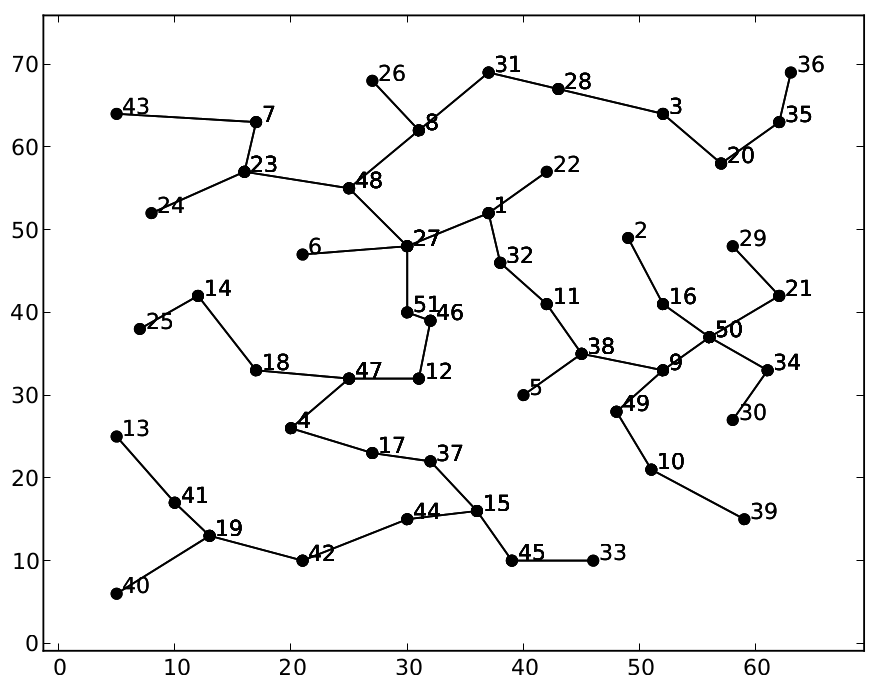
\includegraphics[width=14cm]{gfx/eil51_mst}
        \caption{Minimaler Spannbaum der TSP Instanz eil51 (TSPLIB)}
        \label{img:eil51_mst}
\end{figure}


%TODO: Bilder einfügen, um die Vorgehensweise aufzuzeigen?

\subsection{Minimales Perfektes Matching - Blossom V}
%TODO: Genauer beschreiben
Das minimale Perfekt Matching wird mittels Blossom V Algorithmus berechnet. Der Blossom V Algortihmus ist eine Weiterentwicklung des bekannten Blossom Algorithmus, der 1965 von Edmonds vorgestellt wurde.
Für diesen Algorithmus wird eine bestehende Implementation verwendet. 

\begin{figure}[H]
        \centering
        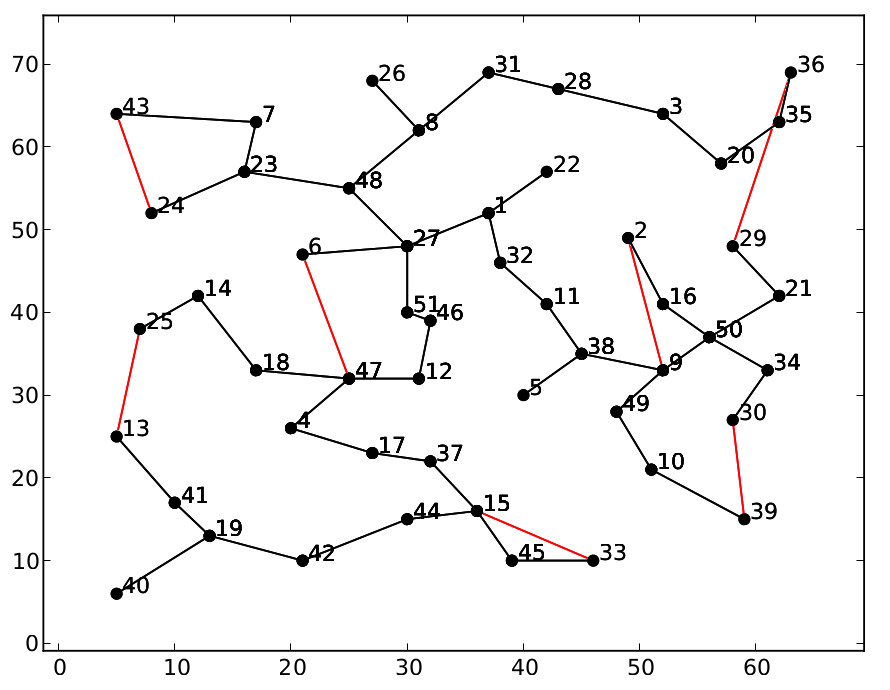
\includegraphics[width=14cm]{gfx/eil51_pm}
        \caption{Minimales Perfect Matching (rot) auf den ungeraden Knoten des MST (schwarz)}
        \label{img:eil51_pm}
\end{figure}

\subsection{Eulerkreis - Hierholzer}
Die Berechnung des Eulerkreises wird mittels Algorithmus von Hierholzer zurück. Dieser wurde 1873 in der postum veröffentlichten Arbeit "`Über die Möglichkeit, einen Linienzug ohne Wiederholung und ohne Unterbrechung zu umfahren"'\cite{hierholzer73} beschrieben.

Der Algorithmus basiert auf der Idee, dass, wenn man in einem eulerschen Graphen einen beliebigen Kreis findet, die verbleibenden Kanten wiederum einen Kreis enthalten. Somit werden die gefundenen Kreise zusammengefügt, bis schlussendlich alle Kanten im Kreis enhalten ist und somit der Eulerkreis gefunden wurde.\footnote{vgl. \cite{krumke05} Seiten 46-48}

%TODO: Ist die beschreibung verständnlich?
\begin{algorithm}[H]
    \renewcommand{\algorithmicrequire}{\textbf{Eingabe:}}
    \renewcommand{\algorithmicensure}{\textbf{Ausgabe:}}
    \caption{Algorithmus von Hierholzer}

    \begin{algorithmic}[1]
    \REQUIRE Graph $G$, dessen Knoten alle einen geraden Grad aufweisen
        \STATE Wähle einen beliebigen Startknoten $v_0$
        \STATE Erstelle einen Kreis $K$ ausgehend von $v_0$
        \STATE Entferne alle Kanten von $K$ aus $G$
        \WHILE{$E(G) \ge 0$}
            \STATE Suche Knoten $v_n$ dessen Grad $\ge 0$
            \STATE Erstelle einen Kreis $K_n$ ausgehend von $v_n$
            \STATE Füge $K_n$ zu $K$ hinzu: Alle Knoten von $K_n$ an Stelle des Startknotens von $K_n$ in der korrekten Reihenfolge in $K$ einfügen
            \STATE Entferne alle Kanten von $K_n$ aus $G$
        \ENDWHILE
    \ENSURE Eulerkreis $K$
    \end{algorithmic}
\end{algorithm}

%TODO: Bilder einfügen, um die Vorgehensweise aufzuzeigen?


\subsection{Kürzung Eulerkreis/-pfad zu Hamiltonkreis/-pfad}
Die kürzung des Eulerkreises bzw. des Eulerpfades werden in der Liste der besuchten Knoten alle doppelten Einträge gelöscht.

\begin{algorithm}[H]
    \renewcommand{\algorithmicrequire}{\textbf{Eingabe:}}
    \renewcommand{\algorithmicensure}{\textbf{Ausgabe:}}
    \caption{Kürzung Eulerkreis/-pfad zu Hamiltonkreis/-pfad}

    \begin{algorithmic}[1]
    \REQUIRE Liste $L$ mit den Knoten des Eulerkreises/-pfades 
    \FOR{$i = 1 \to len(L)$}
        \IF{$L[i]$ not in $K$}
            \STATE Füge $L[i]$ zu $K$ hinzu
        \ENDIF
    \ENDFOR
    \ENSURE Hamiltonkreis/-pfad $H$
    \end{algorithmic}
\end{algorithm}

\newpage
\section{Implementation}
Der gesamte Algortihmus wurde in Python 3 implementiert. Lediglich der Blossom V Algorithmus, für welchen eine bestehende Implementation verwendet wurde ist in C++ implementiert.

Für die Knoten, Kanten und Graphen werden eigene Objekte erstellt, die nachfolgend genauer beschrieben werden. 

%TODO: Einleitung: Verwendete Programmiersprache, Unittesting, etc.
\subsection{Datenstrukturen}
\subsubsection{Knoten}

\subsubsection{Kante}
\subsubsection{Graph}
%TODO: Gewichte sind immer int Werte, verweis auf TSPLIB Doku
\subsection{Algorithmen}
\subsubsection{Minimaler Spannbaum}
\subsubsection{Perfecht Matching}
\subsubsection{Eulerkreis/-pfad}
\subsubsection{Kürzung Eulerkreis/-pfad zu Hamiltonkreis/-pfad}
\subsection{Unittests}

\newpage

\section{Berechnungen}
Für die Berechnung werden einerseits Instanzen aus der TSPLIB verwendet, andererseits selbst erstellte Instanzen.
Zuerst wird das Vorgehen für die Berechnung beschrieben, anschliessend werden die verwendeten Verfahren vorgestellt.


\subsection{Vorgehen}
Um die Lösung der Win/Win Strategie mit der exakten Lösung zu vergleichen wird wie folgt vorgegangen:

\begin{itemize}
    \item Berechnung der exakten Lösung mit Concorde für das TSP 
    \item Einfügen einer Dummy-Stadt (Distanz 0 zu allen Städten)
    \item Berechnung der exakten Lösung mit Concorde für HPP 
    \item Beginn und Ende der Route werden als $s$ und $t$ verwendet
    \item Berechnung der Lösung mittels Win/Win Strategie
    \item Vergleich der Win/Win Lösung mit der exakten Lösung
\end{itemize}

Die Implementierung des Graphes als "`dictionary"' hat zur Folge, dass die Knoten nicht sortiert sind. Dies bringt einerseits massive Geschwindigkeitsvorteile, andererseits führt es aber dazu, dass bei der Berechnung der selben Instanz leicht unterschiedliche Ergebnise berechnet werden.

Um eine möglichst repräsentative Lösung für den Vergleich zu erhalten, wird pro Instanz der arithmetische Mittelwert aus 1000 Berechnungen verwendet.
%TODO: Berechnung entsprechend durchführen

\subsection{Genutzte Ressourcen}
\subsubsection{Concorde}
Zur Berechnung der exakten Lösung wird die Software Concorde verwendet. Concorde wurde von David Applegate, Robert E. Bixby, Vašek Chvátal und William J. Cook, den Autoren des Buches "`Traveling Salesman Problem"'\cite{applegate06}, geschrieben.

Es ist sowohl möglich, die exakte Lösung zu berechnen, wie auch Heuristiken zu verwenden. Für diese Arbeit wurde lediglich die Berechnung der exakten Lösung verwendet.

Neben dem Kommandozeilen-Programm für Linux ist auch ein GUI für Windows verfügbar.\footnote{Download unter http://www.tsp.gatech.edu/concorde/downloads/downloads.htm}

\begin{figure}[H]
        \centering
        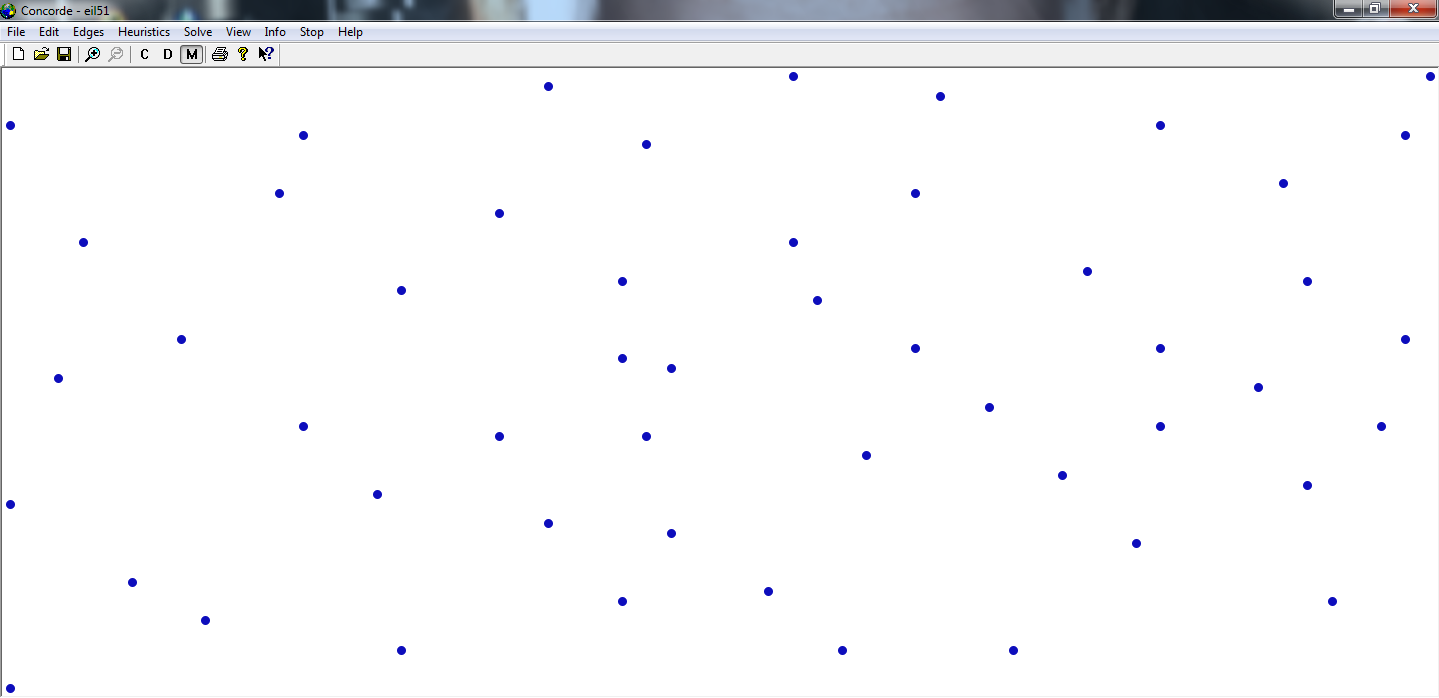
\includegraphics[width=14cm]{gfx/concorde_cities}
        \caption{Concorde stellt eil51 aus der TSPLIB garfisch dar}
        \label{img:concorde_cities}
\end{figure}

\begin{figure}[H]
        \centering
        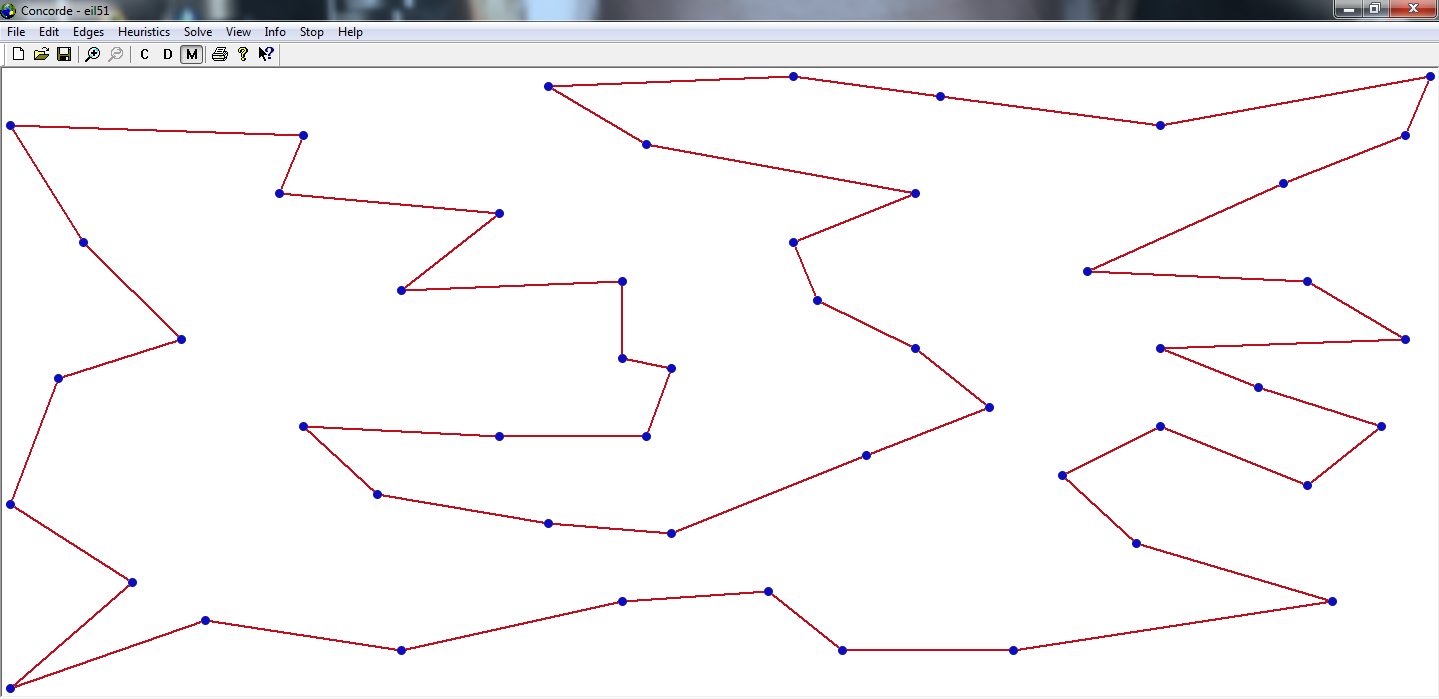
\includegraphics[width=14cm]{gfx/concorde_solution}
        \caption{Concorde hat die exakte Lösung zu eil51 berechnet}
        \label{img:concorde_solution}
\end{figure}

\subsubsection{TSPLIB}
Die TSPLIB ist eine Sammlung von TSP-Instanzen, die 1990 von Gerhard Reinelt erstellt wurde. Sie enthält Instanzen von 14 - 85'900 Städte TSPs und ist wohl die am häufigsten genutzte Sammlung für Berechnungen des Traveling Salesman Problems.\footnote{vgl. \cite{applegate06} Seite 500-505}

Die Instanzen sind in Files abgelegt. Es werden verschiedene Formate unterstützt, unter anderem die Speicherung der Koordinaten im 2 und 3 dimensionalen euklidischen Raum und als Matrix, bei der die Elemente die Abstände zwischen den Knoten darstellt.

\subsubsection{Zufällige Instanzen}

\subsection{Auswertung TSPLIB Instanzen}
\subsubsection{eil51}


        \begin{table}[H]
                \centering
                \begin{tabular}{| l | r |}
                    \hline
                        Anzahl Städte               & 51            \\ \hline
                        Dimensionen                 & 2             \\ \hline
                        Länge optimale Lösung TSP   & 426           \\ \hline
                        Länge Win/Win Lösung  TSP   & 483           \\ \hline
                        Abweichung TSP              & 13.06\%       \\ \hline
                        $s$ und $t$ für HPP         & 36, 40        \\ \hline
                        Länge optimale Lösung HPP   & 403           \\ \hline
                        Länge Win/Win Lösung  HPP   & 459           \\ \hline
                        Abweichung HPP              & 13.90\%       \\ \hline
                \end{tabular}
                \caption{Instanz eil51}
                \label{tab:instanz_eil51}
        \end{table}

\subsubsection{Zusammenfassung}


\subsection{Auswertung eigener Instanzen}
\subsubsection{Zick-Zack}

        \begin{table}[H]
                \centering
                \begin{tabular}{| l | r |}
                    \hline
                        Anzahl Städte               & 39            \\ \hline
                        Dimensionen                 & 2             \\ \hline
                        Länge optimale Lösung TSP   & 7'798         \\ \hline
                        Länge Win/Win Lösung  TSP   & 11'290        \\ \hline
                        Abweichung TSP              & 44.78\%       \\ \hline
                        $s$ und $t$ für HPP         & 1, 39         \\ \hline
                        Länge optimale Lösung HPP   & 7'490         \\ \hline
                        Länge Win/Win Lösung  HPP   & 7'490         \\ \hline
                        Abweichung HPP              & 0\%           \\ \hline
                \end{tabular}
                \caption{Instanz Zick-Zack}
                \label{tab:instanz_zick_zack}
        \end{table}

\subsubsection{Random 3D}

        \begin{table}[H]
                \centering
                \begin{tabular}{| l | r |}
                    \hline
                        Anzahl Städte               & 30            \\ \hline
                        Dimensionen                 & 3             \\ \hline
                        Länge optimale Lösung TSP   & 774           \\ \hline
                        Länge Win/Win Lösung  TSP   & 815           \\ \hline
                        Abweichung TSP              & 3.69\%        \\ \hline
                        $s$ und $t$ für HPP         & 19, 24        \\ \hline
                        Länge optimale Lösung HPP   & 706           \\ \hline
                        Länge Win/Win Lösung  HPP   & 749           \\ \hline
                        Abweichung HPP              & 6.09\%        \\ \hline
                \end{tabular}
                \caption{Instanz Random 3D}
                \label{tab:instanz_random_3d}
        \end{table}

\subsubsection{Zusammenfassung}

\newpage

% bibliography
\bibliographystyle{plain}
\bibliography{bibliographie}
\end{document}
